\chapter{Dekompozycja liniowa}

Redukcja argumentów umożliwia zmniejszenie liczby wejść potrzebnych do realizacji funkcji w układzie kombinacyjnym.
Jednak wyniki uzyskane w czasie takiej optymalizacji nie są ostateczne.
Dalsze zmniejszanie rozmiaru pamięci niezbędnej w procesie generowania indeksów (zgodnie z algorytmem profesora Sasao) można osiągnąć stosując dekompozycję liniową.

Dekompozycja liniowa polega na  łączeniu zmiennych w pary i wprowadzaniu ich za pośrednictwem bramek XOR do głównego układu realizującego detekcję i klasyfikację (czyli indeksowanie) danych.
Jest to istotne,
gdyż prowadzi do dalszego redukowania liczby wejść w generatorach indeksu.
I pewnie z tych powodów dekompozycja liniowa jest intensywnie wykorzystywana w syntezie funkcji generowania indeksów [12-15].

Dobrym przykładem gdzie wyraźnie widać zastosowania dekompozycji liniowej jest funkcja przedstawiona na rysunku numer \ref{fig:required-decomposition}.
Została ona celowo spreparowana w taki sposób,
że wszystkie argumenty są niezbędne.
W takim wypadku redukcja argumentów nie przynosi żadnych rezultatów.
Dodatkowo łatwo zauważyć,
że pierwszy i drugi argument można z powodzeniem zastąpić innym,
będącym wynikiem zwykłej funkcji XOR tych argumentów.

\begin{figure}[H]
\centering
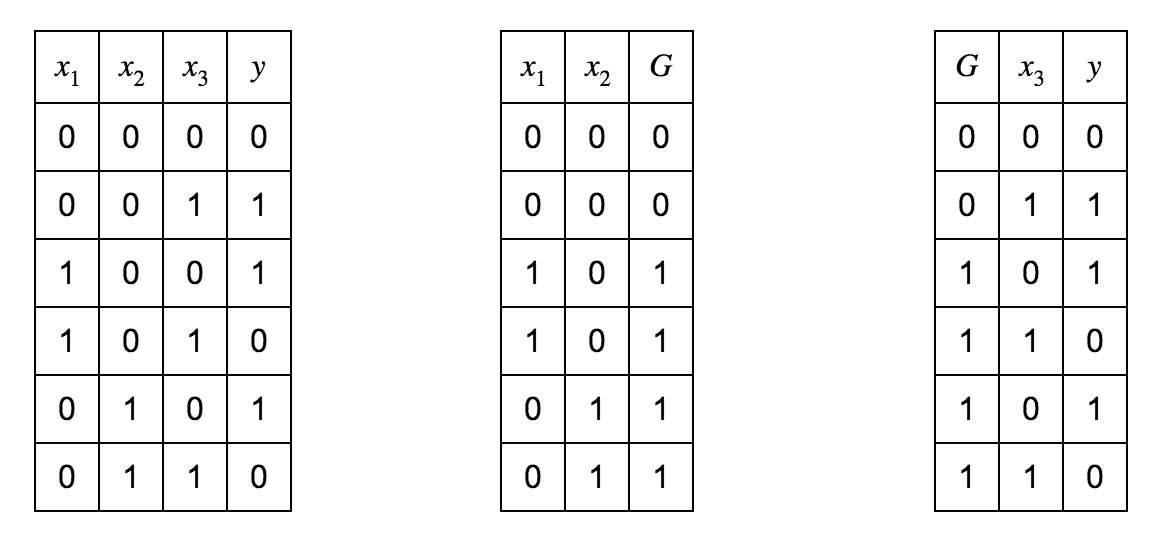
\includegraphics[width = 13cm]{chapter03/required-decomposition.png}
\caption{Przykład obrazujący zlety dekompozycji funkcji z argumentami niezbędnymi (Źródło własne).}
\label{fig:required-decomposition}
\end{figure}

Zmniejszenie rozmiaru pamięci z trzech argumentów do dwóch nie jest zbyt spektakularne i nie miałoby znaczenia w praktycznym zastosowaniu.
Jednak dla innego badanego przypadku nieredukowalnej funkcji 41 argumentowej,
dekompozycja proponowaną w pracy metodą powoduje zmniejszenie liczby argumentów do 7.

Problem generowania indeksów posiada pewną specyficzną własność.
Każdy wektor wejściowy rozważanej funkcji ma inną wartość.
Dotychczasowe rozwiązania problemu dekompozycji liniowej ograniczały się właśnie do takiego przypadku.
Zaprezentowany w tej pracy algorytm jest pod tym względem bardziej uniwersalny.
Można go stosować dla wszystkich funkcji boolowskich o dowolnych wyjściach.

\section{Macierz rozróżnialności}

Pierwszym krokiem w dekompozycji liniowej jest wygenerowanie opisanej wcześniej macierzy rozróżnialności.
Może to oczywiście wiązać się z podobnymi problemami związanymi ze złożonością pamięciową jak w czasie redukcji.
Tak będzie jednak szczególnie przy problemie generowania indeksów.
Charakteryzuje się on tym,
że wszystkie wiersze w funkcji mają różne wartości.
Z tego powodu liczba wierszy po redukcji argumentów nie zmaleje.

Przy zastosowaniu algorytmu w innych problemach,
gdzie różnych wartości funkcji jest stosunkowo niewiele,
na etapie dekompozycji funkcja zredukowana często nie będzie zawierała wszystkich wierszy.
Część z nich po usunięciu redundantnych argumentów będzie zduplikowana.
Dla przykładu badanej funkcji [P5.PLA] na etapie redukcji argumentów nastąpiła redukcja wierszy z 2048 do 128.
Na takim przykładzie łatwo oszacować,
że tablica rozróżnialności wygenerowana na potrzeby dekompozycji będzie miała 250 razy mniejszy rozmiar.

\section{Dekompozycja pojedynczą bramką XOR}

Celem dekompozycji liniowej pojedynczą bramką XOR jest znalezienie takich dwóch argumentów,
które można zastąpić jednym.
Miałby on być wynikiem operacji XOR tych dwóch argumentów.
Bardziej formalnie poszukujemy takich funkcji $G$ i $H$,
które pozwolą na przedstawienie funkcji $F$ w poniższej postaci:
\begin{equation}
F = H( G ( X_a ), X_b)
\end{equation}
gdzie: $X_a = {x_i, x_j}, X_b = X / X_a, G = XOR$

Aby taka dekompozycja była możliwa,
funkcja $G$ nie może powodować utraty niezbędnych informacji.
Inaczej mówiąc po przekształceniu wierszy danych funkcją $G$ nie mogą powstać wiersze sprzeczne.
Ze względu na użycie w dekompozycji funkcji XOR liczba argumentów funkcji $H$ jest mniejsza o jeden od wyjściowej liczby argumentów funkcji F.

Warunkiem poprawnej dekompozycji jest zachowanie wszystkich rozróżnień funkcji $F$.
Istnieje możliwość zapewnienia tego warunku poprzez analizę zawartości macierzy porównań.
Odpowiednikiem pary wierszy sprzecznych na poziomie tablicy rozróżnialności jest wiersz samych zer.
Dzieje się dlatego,
że wiersze sprzeczne mają identyczne wartości na wszystkich pozycjach,
więc operacja XOR,
używana przy tworzeniu macierzy zwraca same zera.

Dekompozycję liniową bramką XOR w celu weryfikacji jej poprawności można przeprowadzić zarówno bezpośrednio na funkcji F,
jak i powstałej na jej podstawie tablicy rozróżnialności.
Jest tak ze względu na to,
że operacja XOR,
użyta przy tworzeniu tablicy rozróżnialności i dekompozycji,
jest przemienna.
Inaczej mówiąc,
kolejność zastosowania dekompozycji oraz generowania macierzy jest przemienna,
co zostało zobrazowane na rysunku numer \ref{fig:xor}.

\begin{figure}[H]
\centering
\includegraphics[width = 13cm]{chapter03/xor.png}
\caption{Przykład obrazujący przemienność funkcji xor z generowaniem macierzy rozróżnialności (Źródło własne).}
\label{fig:xor}
\end{figure}

Wartości w pierwszym wierszu macierzy rozróżnialności można wyrazić w następujący sposób:
\begin{equation}
x_{1_{w_1}} \oplus x_{1_{w_2}} \quad oraz \quad x_{2_{w_1}} \oplus x_{2_{w_2}}.
\end{equation}
Operacje wykonane na argumentach w czasie dekompozycji dla dwóch pierwszych wierszy można z kolei przedstawić jako:
\begin{equation}
x_{1_{w_1}} \oplus x_{2_{w_1}} \quad oraz \quad x_{1_{w_2}} \oplus x_{2_{w_2}}.
\end{equation}
Zatem w nowej tablicy rozróżnialności otrzymujemy wartość:
\begin{equation}
(x_{1_{w_1}} \oplus x_{2_{w_1}}) \oplus (x_{1_{w_2}} \oplus x_{2_{w_2}}),
\end{equation}
 co jest równoważne wykonaniu operacji XOR na istniejącej macierzy rozróżnialności:
\begin{equation}
x_{1_{w_1}} \oplus x_{2_{w_1}} \oplus x_{1_{w_2}} \oplus x_{2_{w_2}}.
\end{equation}

Pośrednim warunkiem zachowania spójności danych jest niepowstanie żadnego wiersza samych zer w tablicy rozróżnialności.
Wiersze,
które po dekompozycji bramką XOR zawierają same zera,
musiały przed dekompozycją przede wszystkim zawierać same zera dla argumentów,
które nie uległy zmianie.
Spośród tych wierszy jedynie te,
które zawierają dwa zera lub dwie jedynki dają wiersz samych zer.
W pierwszym wypadku wiersz już wcześniej zawierał same zera.
Czyli już wcześniej dane były sprzeczne.
W drugim wypadku,
kiedy któryś z wierszy zawiera jedynie dwie jedynki dla dekomponowanych argumentów,
następuje faktyczna utrata informacji.
Brak takiego wiersza jest w takim razie warunkiem wystarczającym do istnienia dekompozycji pojedynczą bramką XOR.

\begin{figure}[H]
\centering
\includegraphics[width = 13cm]{chapter03/single-decomposition.png}
\caption{Przykład dekompozycji pojedynczą bramką XOR (Źródło własne).}
\end{figure}

\section{Dekompozycja wieloma bramki XOR}

Na podobnej zasadzie możliwa jest również dekompozycja z użyciem wielu bramek XOR.
W przypadku,
jeżeli wszystkie pary jedynek występują w macierzy rozróżnialności,
możemy przystąpić do szukania brakujących trójek.
Każdą taką trójkę argumentów,
dla której brakuje trzech jedynek pośród wierszy tablicy porównań,
można z użyciem dwóch bramek XOR,
skompresować do dwóch argumentów.
Nowe argumenty przyjmują wtedy postać np. $x_1 \oplus x_2$ oraz $x_2 \oplus x_3$.
Z tym rozumowaniem można postępować dalej.
Brak jakiegokolwiek wiersza w macierzy rozróżnialność można zamienić przy użyciu pewnej liczby bramek XOR na zysk jednego argumentu w końcowej funkcji.
W każdym z tych przypadków operacja XOR wykonywana jest na kolejnych parach argumentów,
czyli pierwszy z drugim,
drugi z trzecim,
trzeci z czwartym itd.

Dowód,
że brak dowolnego wiersza w macierzy rozróżnialności jest warunkiem wystarczającym do istnienia dekompozycji,
sprowadza się ponownie do analizy zmian w macierzy rozróżnialności.
Aby zdekomponowana funkcja pozostała spójna,
w tablicy porównań nie może pojawić się wiersz samych zer.
Czyli nie może istnieć taki wiersz w tablicy porównań,
który w obrębie modyfikowanych argumentów zawierał co najmniej jedną jedynkę,
lecz po dekompozycji zostały w nim same zera.

Dowód przez zaprzeczenie zacznijmy od pierwszej pary argumentów.
Aby w wyniku operacji XOR argumentów pierwszego z drugim powstało 0,
w pierwotnej macierzy porównań musiały znajdować się albo dwa zera,
albo dwie jedynki.

Zacznijmy od przypadku dwóch zer.
Przechodząc do kolejnej pary (2 i 3),
aby otrzymać kolejne zero w wyniku operacji XOR,
ponieważ argument drugi był zerem,
również trzeci argument musiał być zerem.
Przechodząc w ten sposób po wszystkich parach argumentów biorących udział w dekompozycji,
okazuje się,
że wszystkie z nich musiały być zerami.
Z tego wynika,
że w tym przypadku nie została naruszona spójność danych.

Drugim przypadkiem jest para jedynek dla argumentów 1 i 2.
W takim wypadku,
aby para 2 i 3 w wyniku operacji XOR dawała zero,
również argument 3 musiał być zerem.
Podobnie jak w poprzednim przypadku przechodząc przez wszystkie pary otrzymujemy,
że wejściowym wierszem tablicy rozróżnialności,
musiał być wiersz samych jedynek w obrębie dekomponowanych argumentów.
Taka sytuacja również nie mogła mieć miejsca ze względu na sposób wyboru tych argumentów.

Podsumowując,
operacje wykonywane w czasie tak przeprowadzonej dekompozycji nie mają wpływu na spójność danych.
Tym samym udowodniliśmy,
że brak dowolnego wiersza w macierzy rozróżnialności jest warunkiem wystarczającym do istnienia dekompozycji liniowej.

\begin{figure}[H]
\centering
\includegraphics[width = 13cm]{chapter03/multiple-decomposition.png}
\caption{Przykład dekompozycji dwoma bramkami XOR (Źródło własne).}
\end{figure}

\section{Dekompozycja wielokrotna i wielopoziomowa}

Problem dekompozycji liniowej nie kończy się na znalezieniu pojedynczej dekompozycji.
Dekompozycję można przeprowadzać wielokrotnie tworząc kaskadę jak na rysunku numer \ref{fig:multiple-levels}.

\begin{figure}[H]
\centering
\includegraphics[width = 5cm]{chapter03/multiple-levels.png}
\caption{Przykład dekompozycji wielopoziomowej (Źródło własne).}
\label{fig:multiple-levels}
\end{figure}

W takim przypadku wejściem niektórych bramek XOR są wyjścia poprzednich.
Wartość na wyjściu takiej kaskadowej bramki przyjmuje wtedy postać:
\begin{equation}
(x_1 \oplus x_2) \oplus x_3
\end{equation}
Co jest równoznaczne użyciu bramki XOR o trzech wejściach.
Z tego powodu schemat z rysunku numer \ref{fig:multiple-levels} można uprościć do postaci przedstawionej na rysunku numer \ref{fig:multiple-entries}.

\begin{figure}[H]
\centering
\includegraphics[width = 5cm]{chapter03/multiple-entries.png}
\caption{Przykład dekompozycji wielokrotnej (Źródło własne).}
\label{fig:multiple-entries}
\end{figure}

Jest to istotne,
ponieważ dzięki takiej własności operacji XOR i wykorzystaniu bramek o wielu wejściach,
nigdy nie powstaną długie ścieżki krytyczne.

\section{Algorytm}
- rekurencja, wytłumaczenie schematu dekompozycji przy rekurencji
- zapis w pseudokodzie
- przykład

Kroki:
Generowanie tablicy rozróżnialności
Poszukiwanie brakujących zbiorów n-elementowych w macierzy porównań (n=2)
Jeżeli nie znaleziono
Koniec jeżeli n >= liczba kolumn
Powrót do punktu 2 i poszukiwanie brakujących zbiorów o jeden liczniejszych
Modyfikacja danych oraz zapamiętanie znalezionej dekompozycji
